\documentclass[a4paper, 10pt]{article}
\setlength{\topmargin}{-0.8in}
\setlength{\textheight}{9.5in}
\setlength{\oddsidemargin}{-.13in}
\setlength{\textwidth}{6.5in}

\usepackage{multirow}
\usepackage{float}
\usepackage{array}

\usepackage{datetime}

\newdateformat{mydate}{\monthname[\THEMONTH] \THEYEAR}

\newcolumntype{L}{>{\centering\arraybackslash}m{3cm}}

\usepackage{graphicx}
\graphicspath{{images/}}

\begin{document}


\LARGE\title{User Modeling in search for People with Autism}

\LARGE\author{Author: \textbf{Esha Massand}, Supervisor: \textbf{Keith Mannock}\\
\\
Birkbeck, University of London\\Department of Computer Science and Information Systems\\\\\\Proposal submitted in partial fulfillment of the requirement for the MSc in Computer Science\date{\mydate\today}
\\\
}

\normalsize


\maketitle

\begin{center}

\section*{Abstract}
This project proposal describes my preliminary research in developing and building a prototype system to aid/assist users with searching the web. The user group under consideration are those diagnosed with Autism. The proposed system will focus on modelling user interactions with the search process and developing a user profile for this category of users, integrating insights from the core features of Autism into the model. The prototype will be developed as a web application, utilising a novel user interface component, and applied to search results returned from a synthesis of three leading existing search engines. The project will provide insights into the needs and wants of individuals with Autism within search, and enable future development and intervention within these information streams.\\

\end{center}

\begin{verbatim}





















\end{verbatim}

This proposal is substantially the result of my own work, expressed in my own words, except where explicitly indicated in the text. I give my permission for it to be submitted to a Plagiarism Detection Service. This proposal may be freely copied and distributed provided the source is explicitly acknowledged.

\begin{center}
word count, not including references: 3294 words.
\end{center}

\clearpage
\tableofcontents

\section*{Abbreviations}
\begin{tabular}{l l }
API & Application Programming Interface\\
ASD & Autism Spectrum Disorder\\
DSM & Diagnostic and Statistical Manual\\
GCS & Google Custom Search\\
HCI & Human Computer Interaction\\
JSON & JavaScript Object Notation\\
KWIC & Key Word In Context\\
LEAP & LEAP Motion Controller\\
RIFT & Oculus Rift Virtual Reality Head Mounted Display\\
TDD & Test Driven Development\\
UI & User Interface\\
UX & User Experience\\
VR & Virtual Reality\\
\end{tabular}

\section*{Definitions}
\begin{tabular}{l p{15cm}  }
Autism & Autism is amongst the most common neurodevelopmental condition and it is currently estimated that 1/68 children meet criteria for Autism Spectrum \cite{CDC}. Autism is five times more common amongst boys than girls (1/42 boys, and 1/189 girls). According to the Diagnostic and Statistical Manual (2013), Autism is characterized by persistent and early deficits in reciprocal social interaction and repetitive behaviours. Individuals vary from high functioning to low functioning (along a spectrum), with behaviours emerging around 2 to 3 years of age.
\end{tabular}
\clearpage

\section{Introduction \& Background}\label{prob}
People with Autism are less context-sensitive and prefer a more detail-focused processing style \cite{mottron}, and they form web-search queries differently to the typical population. Individuals with Autism are also less likely to engage in a relational (hierarchically organized) style of processing \cite{bowler} suggesting that relating information in a hierarchically organised framework is less likely. Hierarchical organisation implies flexibility and mental-shifting, as a simple example, in a search for 'apple', it would imply awareness that the word is related to 'pear' but also to 'fruit'. Awareness of this latter relation also suggests awareness that 'apple' is related to 'pomegranate'. This is a simple example, but these associations can get very complex, very quickly. Generally speaking, individuals with Autism prefer, and are more likely to engage in an item-specific processing style, and, whilst intelligent cognition is definitely possible, web-search queries are more likely formed of first-order associations\footnote{There is a great deal of individual variability in the Autism Spectrum.}.To address this issue, the current project aims to build a user model within search for individuals with Autism. 

\begin{figure}[H]
\begin{center}
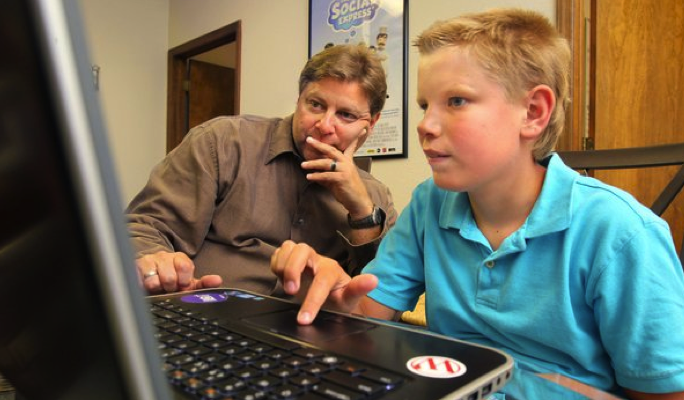
\includegraphics[scale=0.2]{person}\\
\caption{Current web navigation and information retrieval \cite{person}}
\end{center}
\end{figure}

\subsection{The Role of Context Within Search} \label{the problem}
It is unlikely that any given page on the web will contain a word or phrase that means exactly (or nearly) the same as another word or phrase in that language (e.g., shut and close). How is it then that your search engine picks these phrases to mean the same thing, and returns them synonymously in the results of your query? Well, quite simply put, with the use of a thesaurus, synonyms and by virtue of the fact that each of their neighbouring words and associations are similar. These are indirect, higher-order associations, and provide the context in which the search engine index keywords.

Most search engines apply user models to refine user search queries. For example, adaptive search engines use assumptions about users from specific subgroups to tailor search results accordingly. These models can often lack specificity for users, or groups of users \cite{usermodel}.  Based on the Psychology literature, autistic traits show the same etiology in the general population, but at the quantitative extremes \cite{robinson}. This implies that the parameters of general user models could be adjusted to successfully cater towards the extremes of the population, and therefore people with Autism \cite{bonel}. Yet, despite Autism being amongst the most common neurodevelopmental condition (1/68 children meet criteria for Autism Spectrum \cite{CDC}), no user model has yet been developed for Autism. 

According to the Diagnostic and Statistical Manual \cite{CDC}, Autism is characterized by persistent and early deficits in reciprocal social interaction, so interaction with computers is prominent in this group. It is also well established that individuals with Autism are more engaged when using technology that is receptive and interactive (e.g., games, responsive consoles, motion controlled devices) compared to technology that is not \cite{motioncontrollerforautism}, this project will combine interactive, motion recognition hardware with search to also improve the UI (user interface) of search for individuals with Autism.

\subsection{The Problems with Current search Tools for People with Autism}\label{What should search offer people with Autism}

The Internet is one of the largest resources of information. Search engines allow users to collate hundreds of links on a single topic, using only a few words or phrases. The typical user sorts the returned results into 'relevant' or 'irrelevant' categories, flexibly shifting (mentally) between one result and the next, to determine the relevance of each page returned by the search engine. Search allows the user to assimilate the information on the page into their knowledge and is an important learning tool. For people with Autism, the requirement is no different; search is an important tool for learning. However, current search is not adequate because the requirement to 'mentally shift' between results is harder for people with Autism \cite{disengagement}. The information is therefore harder to assimilate and learn for them. 

Individuals with Autism have poor attention \cite{attention}. The static 2-dimensional interface of many current search engines are unlikely to maintain adequate (sustained) interest levels. Individuals (and especially teenagers) with Autism spend a substantial amount of their time using computers, web, portable or console devices \cite{Shane and Albert}, as they find these more stimulating and attention-grabbing. For these individuals, computer-based technologies provide a stable, consistent learning environment that can be customized \cite{moore}. Furthermore, motion recognition devices can be programmed to make consistent responses to environmental triggers. These controlled and interactive environments have shown promise for improving social communication skills and reducing repetitive behaviours \cite{gameshealth}. For the current project a motion-controlled learning environment will be bolstered to improve attention within search for people with autism. 

Current search is text-ridden and extremely verbal. This is a problem for people with Autism because they have a stronger visual memory \cite{fabienne} than verbal memory. A more visually-oriented approach to search (reducing the 'verbal working memory' load \cite{workingmem}) is a more appropriate way to bolster the strength of visual memory in people with Autism.

The three top search engines are Adaptive (Google) or Personalised (Yahoo, Bing). They associate each user with a HTTP-cookie containing information such as login (gender, age), preferences (languages, interests) and previous search history (e.g., Google, Bing, Yahoo) \cite{googlepersonalised, yahooadaptive, bingadaptive}. This allows the website to ‘remember’ what buttons the user clicked on, or sites visited, and allows the search engine to return results that are highly related to pages that the user visited through previous searches. Although adaptive search seems to have significant user benefit in terms of relevance of returned pages to the user, it decreases the likelihood that the user encounters new information, biasing the results towards the users location and previous site traffic.  This has the unwanted effect of creating a filter bubble \cite{Pariser}, which is argued to close us off from important and relevant information. It creates a personal ecosystem of information for one user, giving the impression that their self interests are all that exist \footnote{The filter bubble also has potential privacy problems, as the user may be unaware that the search has been specifically tailored towards their interests and they wonder why things that they have previously searched for have become more and more relevant. There are search engines that have attempted to address this unwanted effect, by not tracking or saving user information (e.g., DuckDuckGo.com). As users are not linked to their search queries, it limits them being targeted by adverts related to their previous searches.}. Unfortunately the filter bubble may positively reinforce restricted interests in Autism as the user constantly receives feedback about their previous (idiosyncratic and personalized) searches without being able to break out of that repetitive loop. 

Research suggests personalization also increases ‘background noise’ relative to the search results \cite{briggs}, with a carry-over effect in personalized search, where prior search influences the results from subsequent searches \footnote{It should be noted that personalization of search results generally takes a lower priority for the ranking algorithms than the URLs ranked top in terms of their relevance for the search query.}. This carry-over may be particularly disadvantageous for people with Autism (some of whom already have restricted and repetitive interests) as it muddies their search space. To produce a search tool specifically tailored to reduce the filter bubble effect in Autism, widen the information gateway and reduce the possibility for restricted and repetitive searches, the weighting on previous search results will need to be reduced. This is something I will investigate in the project, particularly for individuals who identify restricted or repetitive interests. For these users, it would limit the possibility that they get trapped in a spiraling loop of ever-narrowing user-relevant information and over-personalization of self-reinforced information ecosystems.

\section{Aims and Objectives} 
As part of my project I propose to build a user model of Autism, for a motion-controlled, web search. See Figure ~Figure\ref{vision} for the envisioned UI interface of the project, and Figure ~\ref{architec} for the proposed architecture. The core and non-core features of the application are given below. I elaborate on each of the key features in the following sections. 

\begin{figure}[H]
\begin{center}
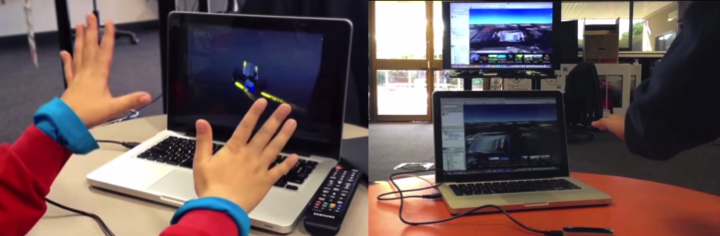
\includegraphics[scale=0.35]{vision}\\
\caption{Envisioned UI interface component for the project \cite{leap}.}
\label{vision}
\end{center}
\end{figure}

\subsection{Proposed Architecture}\label{proposed}
\begin{figure}[H]
\begin{center}
    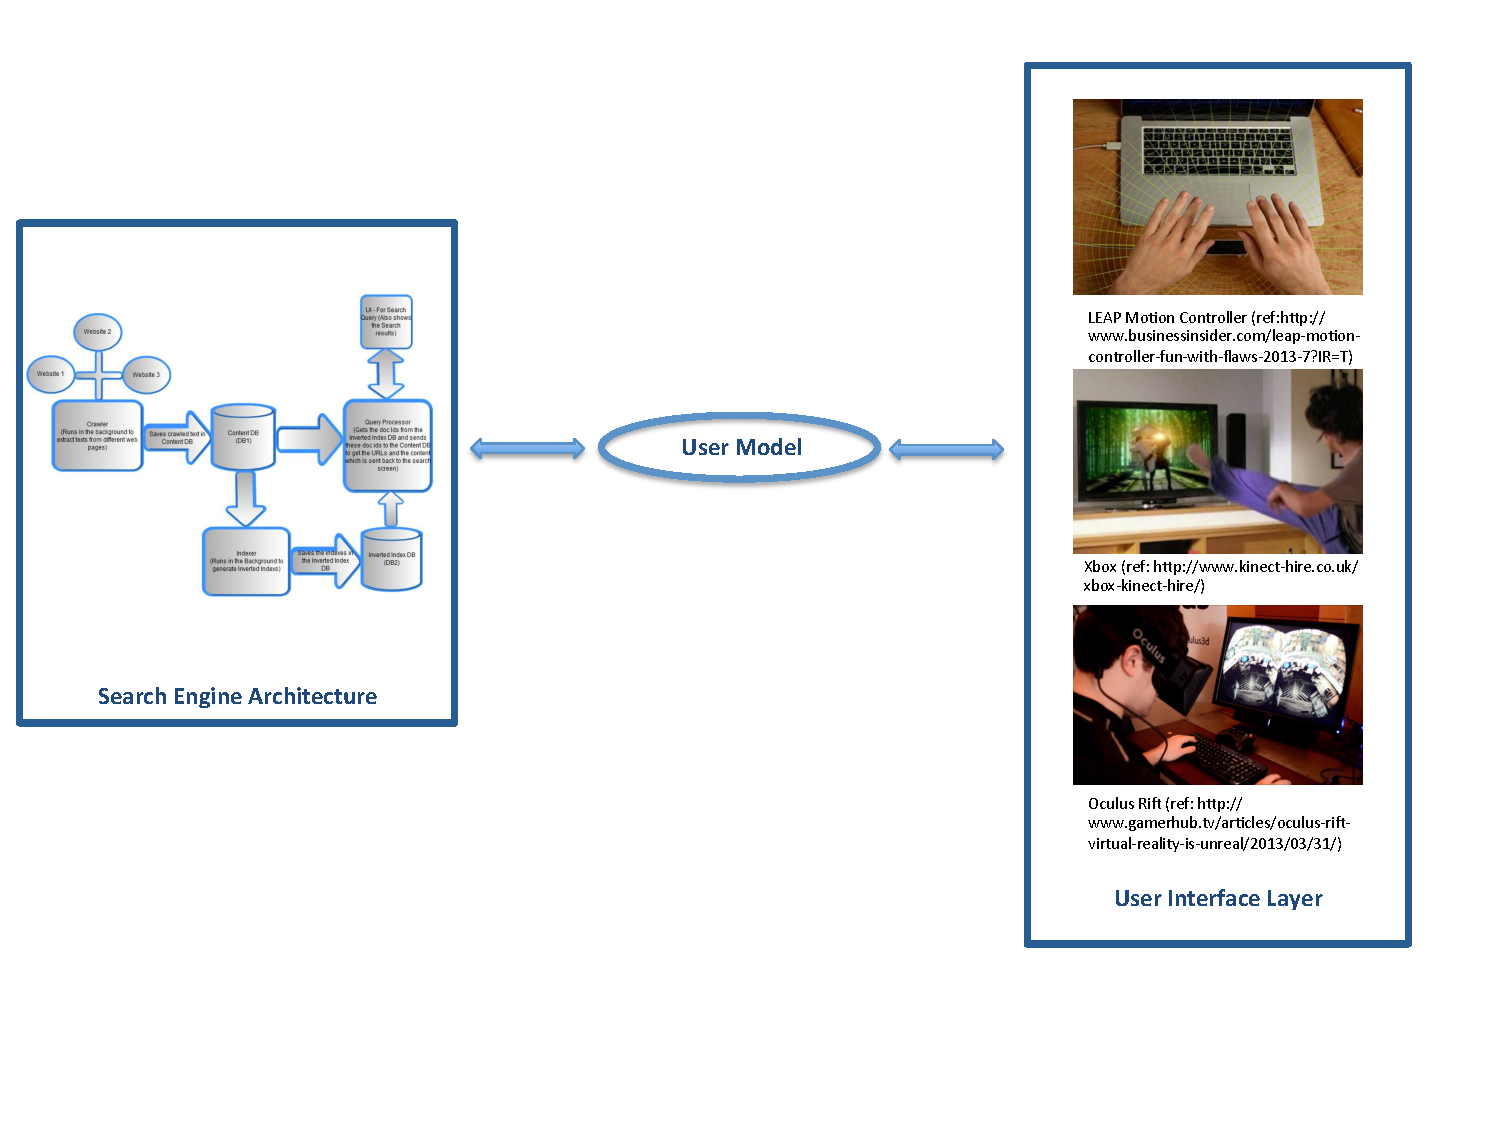
\includegraphics[scale=0.3]{searchEngArchi}
    \caption{The User Model will be applied to existing search Engine Architecture\cite{seimage}, and be integrated with Motion Controlled interfaces such as the Rift, LEAP and Kinect \cite{rift, leap, kinect}.}
    \label{architec}
\end{center}
\end{figure}


\subsubsection{Core Features}\label{core}
\begin{enumerate}
\item  \textbf{A combination search (web application) that synthesises the results from three of the largest and most popular engines; Google, Bing and Yahoo \cite{adam}.}

\item \textbf{The design and implementation of a user model of Autism to filter user search results. This will be a \textit{stereotyped} model, i.e., some characteristics of the model will be based upon the user's demographic data, other characteristics will be inferred from the Autism subset of users (see Section ~\ref{usermodel} for an explanation of the different types of user models.)}

\item \textbf{Key Word In Context search; returning query terms in context, within small snippets (not verbally-overloaded).}

\item \textbf{Prioritisation of results which have first-order semantic relations to the query words (see Section~\ref{the problem}), i.e., they appear in matched context to the search query.}

\item \textbf{Motion controlled UI (see Section \ref{hardware}).}
\end{enumerate}

\subsubsection{Non-core Features}
\begin{enumerate}

\item Implement a higher ranking for pages with most images. 
\item Use of WebGL and the three.Js library for 3D UI .
\item Compatibility with other motion controller devices (e.g., head-mounted devices).

\end{enumerate}

\section{Plan for Developing the Solution}\label{sol}
The first part of the project involves building a synthesis of search engines. In my research I considered several existing solutions, these included: (1) \textbf{'Bing vs. Google'}\cite{bingvsgoogle}, which presents search query results from Bing and Google side-by-side, allowing the user to make a comparison, and providing the experience of navigating both search pages simultaneously; (2) \textbf{'Qrobe'}\cite{qrobe}, which combines three search engines’ results (Google, Bing and Ask) on one page, but the user can also search ‘web’, ‘images’ or ‘popular’; (3) \textbf{'AskBoth'}\cite{askboth} combines both Google and Bing results, integrating a section in the middle, dedicated to a twitter feed; and (4) \textbf{'Specra'}\cite{specra}, which attempts to include user preferences by combining results from Google, Bing and Yahoo and allowing users to assign 'weights' to each engine. These existing solutions are limited, however, as the number of personal preference options is very limited. In addition, there is often double (or triple) the amount of verbal information on the results page, resulting in verbal (and cognitive) overload for users with Autism, as well as redundancy (near-duplicates). Furthermore, where an RSS-feed such as twitter (or other social media) may add to the aesthetics and user experience (UX) for a typical user \cite{social}, for individuals with Autism who prefer rigid routines, continuous updates are distracting and sub-optimal \cite{disengagement}. I therefore plan to synthesise the results from search engines using their individual Application Programming Interfaces (API) (which I discuss in the proceeding sections). The rest of this planning section outlines how each of the core features listed above in Section~\ref{core} will be developed.

\subsection{Building the Combination search Engine: Core Feature 1.} 
The three most popular search engines, Google (unique monthly visitors = 1,100,000,000, query volume = 64.5\% ), Bing (350.000.000, 12.8\%) and Yahoo! (300,000,000, 64.5\%) were selected \cite{ebiz, adam}. Other search engines were not included, to limit redundancy of the search results returned.

To combine search results, I will use API’s provided by Google, Yahoo and Bing, as this is more efficient than inspecting the source code for every query result-page. For Google search results, the \textbf{Google Custom Search API} (GCS), (available in Java) will be used to create a personalised search engine. GCS requires a domain name and server at configuration, and provides a consumer key and secret, which are hardcoded in the application. Using the API I will extract image search results, page dates, formatting dates, custom snippets, and sort and filter the results. For Yahoo search, the \textbf{Yahoo BOSS Java API} will be used, for Bing, the \textbf{Bing search API}. These APIs offer similar functionality as the GSC\footnote{The APIs alone may not be comprehensive for textual-search (KWIC), and an addional library may be required (see Section~\ref{apache}).}. Each costs \$0.01/search (max 5000 searches/month). Figure ~\ref{apistream} shows the input of these API into a synthesised stream.

\begin{figure}[H]
\begin{center}
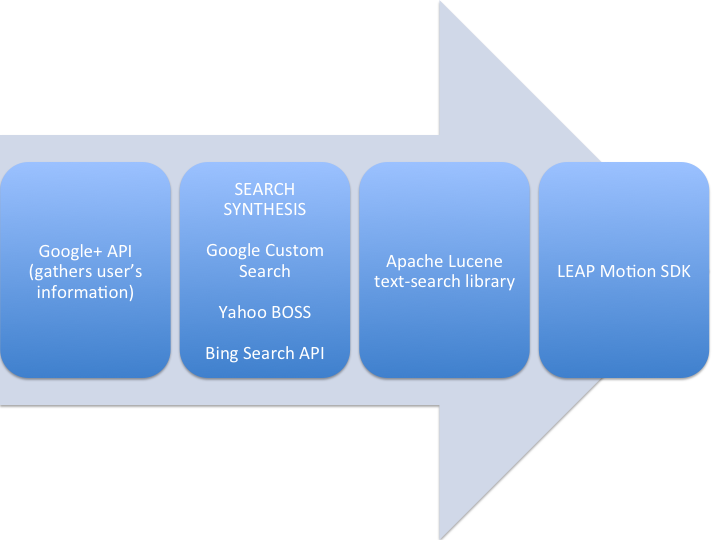
\includegraphics[scale=0.3]{apistream}\\
\caption{Usage of APIs proposed for the project.}
\label{apistream}
\end{center}
\end{figure}

\subsection {Building a User Model of Autism: Core Feature 2}\label{usermodel}
A user model (or a collection of information associated with a particular user, usually a data structure), will be developed so the current system can adapt/customise its behaviour in line with user needs, and be better informed about how to behave in various circumstances, improving the human-computer interaction experience. In the current case, the user will be required to set up a Google+ account, where their basic information (demographics, needs, preferences, likes, dislikes, goals, plans, knowledge, and skill), will be gathered. They will authenticate their Google+ account with the web application to start the formation of their data model. I will access these data via the \textbf{Google+ API}, which includes methods to access 4 resource  types; People, their Activities, Comments and Moments. A person is represented with many fields in Google+, including name, gender, title, occupation and so forth. I will ask users to enter their Autism diagnostic information in the 'about me' section on their profile. This information will be parsed at a later stage and feed into the user model. Information about web-search history for any individual user can be obtained from the browser history. 

User models fall into 4 main categories. They can be \textit{static/unchanging} (i.e., no algorithms update the model about the user's changing preferences), or \textit{dynamic} (representation of the user with their up-to-date changes in interests, and interactions with the system). User models can be highly \textit{adaptive} and model the user on their own, however, this requires a large amount of data before implementation. \textit{Stereotyped} user models overcome this problem by inferring characteristics about a user from data gathered from other users within that distinct subset. These are the most advantageous in the current case as they can be built quickly using clusters of characteristics of groups of individuals. I will have limited data to work with at the start of the project (only basic information gathered via a registration process, and diagnostic information). So, to address core feature 2, I will build a stereotyped user model (see Figure ~\ref{usermodelconstruct} for an example of what constructs may feed into the user model) , around a cluster of characteristics of well-researched cognitive aspects of Autism (see Section~\ref{What should search offer people with Autism} for a list).


\begin{figure}[H]
\begin{center}
    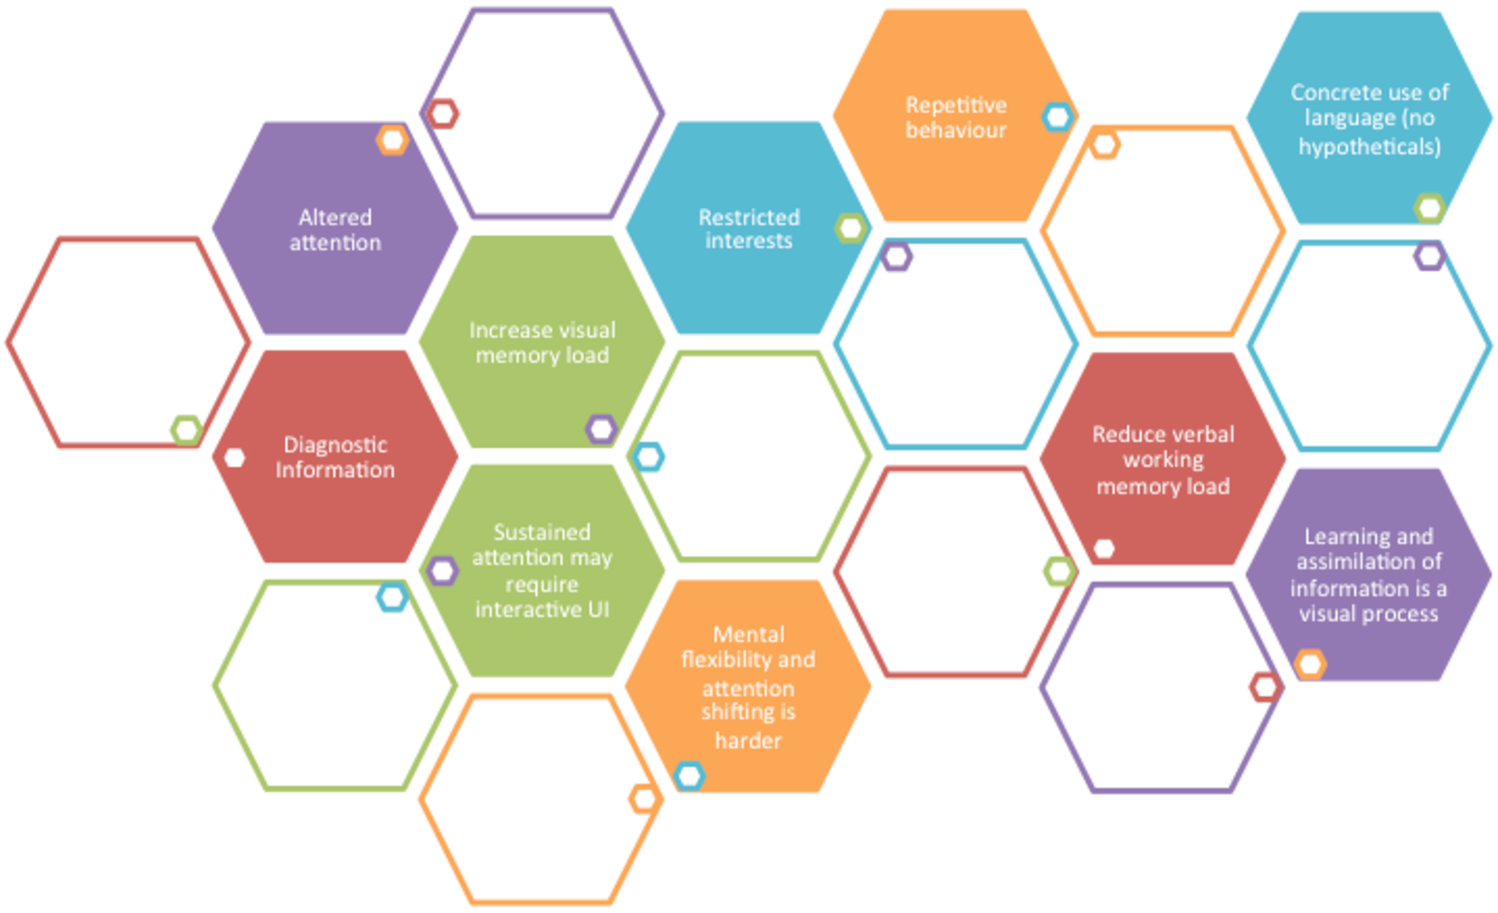
\includegraphics[scale=0.5]{usermodelconstruct}
    \caption{Hypothetical example of features that may feed into the user model. White spaces represent unknowns/inferred/assumptions in a stereotyped user model.}
    \label{usermodelconstruct}
\end{center}
\end{figure}


\subsection{Key Word In Context Search: Core Feature 3}\label{apache}
To identify results which contain the Key Word In Context (KWIC)\cite{kwic} (core feature 3), the \textbf{Apache Lucene Library} (hereafter referred to as 'Lucene') will be used. Lucene is a text-search library (written in Java), providing powerful, scalable, accurate and efficient algorithms to search textual data. The API offers the possibility to carry out phrase, wildcard, proximity and range (distance-of-words) queries. Using the library it will be feasible to ascertain whether the key word appears in a context matched to the user's search query. One possibility is to use the \textbf{lucene.search.highlight} package, and the \textbf{WeightedSpanTermExtractor} class, to extract \textbf{WeightedSpanTerms} from a query, based on whether the query terms appear in a \textbf{TokenStream} (the snippet in this case). This will essentially parse the text to extract the key words in a small surrounding snippet. Each word in the TokenStream is assigned a weight, and if their combined weights sum to above a threshold, this snippet will be returned to the users results page. Snippets whose terms do not exceed the threshold will not be returned. The threshold will be higher than what is currently used in search, and the snippets in the TokenStream will be shorter, to reduce the number of results returned to the user and lessen the cognitive and verbal load of the results page. This is somewhat equivalent to a reduction in the \textit{recall} and increase in \textit{precision} of the search engine. For example, if the user queried 'fluffy cats', instead of the search results returning hundreds of results (containing 'fluffy' and 'cats'), only those where the words appear in proximity to each other (i.e., in the small snippet), and in the top ranking positions of the page (e.g., the title), would be returned. 

\subsection{Identifying First-Order Semantic Relations: Core Feature 4}\label{apache}
The Lucene library will be used to identify and filter search results which contain first-order semantic relations to the query. I will acheive this by overriding the computations of the components in the Lucene \textbf{Similarity} class, and working with the output from the \textit{Practical Scoring Function} (see the Lucene Similarity Class documentation \cite{similarity}), which is at the root of, and directly connected to, the classes and methods in the library. Simply put, the scoring function builds a Vector Space Model (a model to represent the text documents), and calculates the cosine similarity between two documents based on the term frequency - inverse document frequencies\footnote{Term frequency–inverse document frequency is a numerical statistic that is intended to reflect how important a word is to a document in a collection or corpus}. For a full explaination, and derivation of the function, see \cite{similarity}. I will alter these computations to modify the Lucene scoring system in line with the aims of core feature 4. 

To support the alterations in the Lucene scoring system, I will also define fields for sections of a document (e.g., title, heading or subheading number, paragraph number), and apply a 'ranked search' algorithm. For example, if a user queried 'Pythagoras Theorum', a document could be given a higher rank if 'Pythagoras' appeared in the first subheading compared to the last paragraph of the document. One way to acheive this would be by using the Lucene \textbf{Field} class and the \textbf{setBoost} method within the scoring function. 

\subsection{Motion-Controlled UI: Core Feature 5}\label{hardware}
Two options were available for use with the current project, the \textbf{Oculus Rift Virtual Reality head mounted display} (the 'Rift') and, the \textbf{LEAP Motion Controller} (the 'LEAP'). Both have accurate timing, and work well with the combinatorial configuration of senses (sight, hearing and touch). As this is a tool to be used with individuals with Autism, who have increased sensitivity to touch, the sensation and imposition of the Rift was considered to be too overwhelming, and the LEAP was favoured. The LEAP is also more affordable for users to integrate with search at home. 

The LEAP will recognize and track hands, fingers, finger-like tools, positions, motions and gestures using infrared light and optical sensors along the x, y and z cartesian coordinate system. The controller has a 150-degree field of view, and can operate in a range of 1 inch to 2 feet. The API works with distance in millimetre resolution. Time is measured in microseconds, speed in mm/s and angles in radians. The LEAP will use the \textbf{Frames} class, to represent tracked entities, and the motion data will be recorded as a set of frames (stored, read-only) containing the detected motion. I will create frames by calling the Controller.frame(), up to 60 frames can be held in the history buffer. If there are resource contrainsts, frames can be 'dropped'.

\begin{figure}[H]
\begin{center}
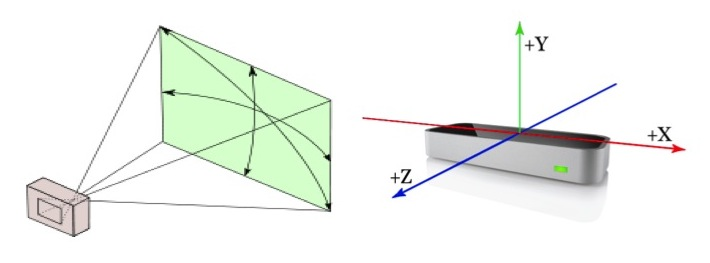
\includegraphics[scale=0.4]{leap}\\
\caption{The LEAP controller, with 150 degree view \cite{leap}}.
\end{center}
\end{figure}

The \textbf{LEAP Motion SDK} will get tracking data from the LEAP Motion Service. A WebSocket interface, allows LEAP Web Based applications, and a WebSocket server listening in on http://127.0.0.1:6437\footnote{The user will be able to enable or disable the WebSocket server.}. The server will send tracking data in JSON messages and the application will send configuration messages back. This is the process I will use to establish connection to the server and consume the JSON messages \cite{leap}. 

For hand movements the \textbf{Hand} class, will return information about the position of fingers, and arm (left/right). The Hand palmNormal() method and direction vectors define the orientation of the hand \cite{leap}. The software will use parts of visible hands, internal models and previous observations to form a model of the hand. I will use the Hand.confidence() method for a rating of how well the observed data fit the internal model \cite{leap}.

\begin{figure}[H]
\begin{center}
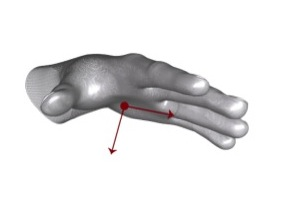
\includegraphics[scale=0.4]{palm}\\
\caption{Hand palmNormal() method \cite{leap}}
\end{center}
\end{figure}

The \textbf{Arms} class will return information about orientation, length, width and end points of movements. The LEAP controller software bases these return measurements on previous observations of the user, and using typical human proportions. Similarly, \textbf{Finger} characteristics are based on the anatomy of the hand, and recent observations. 

\begin{figure}[H]
\begin{center}
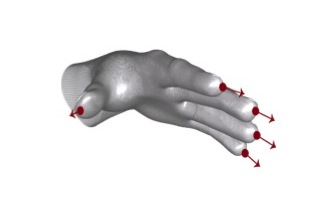
\includegraphics[scale=0.4]{fingers}\\
\caption{Finger tip position and direction are given as vectors \cite{leap}}
\end{center}
\end{figure}

\textbf{Tools} can represent any real object (noun), but are longer, straighter and thinner than fingers, and must be cylindrical. The LEAP can also recognise certain movement patterns, i.e., \textbf{Gestures} (CircleGesture, KeyTapGesture, ScreenTapGesture and SwipeGestures) allowing the user of the system to indicate an intent.

The user will be able to navigate the application with a range of movements involving Hands, Fingers, Gestures and Tools, fulfilling the aims of core feature 5.

\subsection{ThreeJs Library: Non-Core Feature}
ThreeJs is a Javascript library enabling WebGL-3D in the web browser, for hardware-accelerated 3D graphics without installing software. Time permitting, ThreeJs will be used to integrate 3D interfaces with the application and motion controller. This will improve the experience of embodiment, UX, and UI for the user.

\subsection{Methodology}
There is a relatively short deadline in which a single developer will research and deliver a system prototype and report. The APIs, technology and areas of development are unfamiliar. As the final product depends on user feedback testing, there is an element of uncertainty about what the final product will be/should look like. These characteristics suggest that the most suitable methodology to deliver the application is an Agile-like Methodology \cite{agile}. I will focus on early development and rapid feedback to make adjustments to the project's direction. This methodology offers the most flexibility and adaptability.


\subsection{Development Languages}
The Google, Yahoo, Bing and Lucene APIs are available in Java. The LEAP SDK sends Frame information in JSON format to Web Browsers. I will use HTML5 for front-end development.

JSON is light weight, language-independent data format, and a good tool for sharing data. Importantly JSON offers faster execution and server-side parsing by storing the data in arrays. Faster parsing is particularly important for sharing the LEAP motion controller data. A drawback of JSON is that it only has limited support tools available, and little error handling capabilities. Java is a platform and operating-system independent language. It offers a simple, dynamic, robust object oriented, and functional language. There is excellent documentation available for the language, with many third party, open source libraries.

I will use Eclipse text editor and attempt to make the application compatible with Google Chrome browser (as it is WebGL-compatible). I will use Git for Version Control. For testing I will use JUnit, JSON Test and Mockito (for user/external dependencies).

\subsection{User Testing}
I aspire to test the application with a group of individuals with Autism. However, it requires time to acquire ethical approval, it is not clear whether I will be able to acheive this before the deadline. If time allows, user testing would include inviting people Autism to use the web application and obtaining their feedback (relevance/explicit feedback, and, implicit feedback, e.g., mouse clicks), as well as qualitative data. We are currently in contact with the National Autistic Society \cite{nas}, and in the process of seeking assistance with locating participants. I could use the Tobii Eye-tracker (from the Department of Psychology, Birkbeck) to gather high resolution eye-tracking data, as users navigate the application. I would then further revise the user model and UI given their feedback, to improve the final application.

\subsection{Unit Testing}
I will be implementing Test Driven Development (TDD)\footnote{The TDD process involves iterating through the write-test-then-write-code process. First writing a test for some functionality, and second, writing just enough production code to make the test pass.} with JUnit (version 4.12), and where there are external dependencies, these will be mock tested using Mockito \cite{mockito}. JSON Test will be used to test JavaScript Object Notation \cite{jsontest}. I will run both unit and regression tests.

\subsection{Challenges/issues, probabilities and mitigation of impact}
The challenges associated with the project, their impact and how I will mitigate them, is outlined in~Table \ref{risks}. 
\begin{table}[H]
\caption{Challenges \& Impact Mitigation} 
\centering
\begin{tabular}{|c | c | p{6cm} | p{6cm} |}
\hline\hline 
Liklihood & Impact & Challenge & Mitigation\\ [0.5ex]
\hline 
LOW & HIGH & API's require significantly high payment & Find/use alternative\\
\hline 
LOW & HIGH & KWIC library does not offer methods needed to achieve goals of contextual text search & See if I can implement the method, or find additional API\\
\hline 
MEDIUM & MEDIUM & Google+ API does not configure a user persona/user model well & Use Facebook or alternative\\
\hline 
MEDIUM & HIGH & LEAP does not integrate with web application & Investigate user forums, contact LEAP to source answers, adjust web application accordingly.\\
\hline
MEDIUM & HIGH & User Model lacks impact and power in search & Plan further development. Modify weights of parameters in the algorithm. Revise the model. \\
\hline 
MEDIUM & HIGH & Not enough turn around time to implement the userfeedback & Develop plan and prototype in time for report submission\\
\hline
HIGH & LOW & Cannot get research participants with Autism to take part in a usability test & 1. Expand age range of interest in attempt to find participants. 2. Drop aim as it is a non-core feature.\\ 
\hline

\end{tabular}
\label{risks} 
\end{table}

\subsection{Project Timeline}\label{plan}
The start date of the project is June 5th 2015, and end date is September 13th 2015. Non-core features will only be completed, time permitting.
\begin{table}[H]
\caption{Project Stages} 
\centering
\begin{tabular}{ | L |c| L |}
\hline\hline 
Dates & Task & Priority\\ [0.5ex]
\hline 
Jun 05 - Jun 12 & Configure relevant API's \& Libraries to domain name/server & MUST\\
\hline 
Jun 13 - Jun 19 & Synthesise search results & MUST\\
\hline 
Jun 20 - Jul 05 & Research \& build user (and data) model of Autism & MUST\\
\hline 
Jul 06 - Jul 13 & Work on configuration with Google+ API & MUST\\
\hline 
Jul 14 - Jul 20 & Apply user model to search& MUST\\ 
\hline 
Jul 21 - Jul 27 & Develop UI & MUST\\
\hline 
Jul 21 - Jul 28 & Develop questionnaire and eye-tracker set up & COULD\\
\hline 
Jul 29 - Aug 05 & Integrate motion controller tools& MUST\\
\hline 
Aug 06 - Aug 13 & Test the model and ask for user feedback & COULD\\
\hline 
Aug 14 - Aug 21 & Revise the user model and UI & MUST\\
\hline 
Aug 14 - Aug 21 & Develop UI with other motion controllers & COULD\\
\hline 
Aug 22 - Aug 29 & Develop UI using WebGL/threeJs library & COULD\\
\hline 
Aug 22 - Aug 29 & Write up project report & MUST\\ 
\hline 
Early Sep (tbc) & Present findings to supervisor & MUST\\
\hline 
Sep 13 & Submit report & MUST\\[0.5ex]
\hline
\end{tabular}
\label{stages} 
\end{table}

\subsection{Concluding Statement}\label{future}
I have proposed to build a system that enhances the experience of searching the web, for people with Autism. This proposal explains how I will first set about constructing a user model of Autism, from user interactions with search, and, from well-understood aspects of cognition in Autism. Second, I will use text/content based libraries to refine search results for this subgroup. Third, I will integrate the final web application with a novel user interface, the LEAP motion controller. I hope these insights will assist with the forthcoming information-overload problem by exploiting user models to turn the masses of information available into a specific set of “information goods”.

\clearpage
\begin{thebibliography}{100}

\bibitem{person} Child Development Institute, http://childdevelopmentinfo.com/family-living/kids-media-safety/children-teens-web-internet-safety/, Retrieved 11 April 2015

\bibitem{mottron} Laurent Mottron, Jacob A. Burack, Johannes E. A. Stauder, Philippe Robaey (1999) Perceptual Processing among High-functioning Persons with Autism. \textit{Journal of Child Psychology and Psychiatry 40}, (2), 203–211. doi:10.1111/1469-7610.00433

\bibitem{bowler}Dermot M. Bowler, Sebastian B. Gaigg, John M. Gardiner (2014) Binding of Multiple Features in Memory by High-Functioning Adults with Autism Spectrum Disorder, \textit{Journal of Autism and Developmental Disorders September 2014, 44}, Issue 9, pp 2355-2362

\bibitem {CDC}Developmental Disabilities Monitoring Network Surveillance (2010) \textit{Centers for Disease Control and Prevention (CDC). Prevalence of autism spectrum disorders: Autism and Developmental Disabilities Monitoring Network, United States. MMWR Surveill Summ.2009; 58}, 10:1–20

\bibitem{robinson} Robinson EB, Koenen KC, McCormick MC, et al. Evidence That Autistic Traits Show the Same Etiology in the General Population and at the Quantitative Extremes (5\%, 2.5\%, and 1\%). Arch Gen Psychiatry. 2011;68(11):1113-1121. doi:10.1001/archgenpsychiatry.2011.119.

\bibitem{bonel} Bonnel, A; Mottron, L; Peretz, I; Trudel, M; Gallun, E; Bonnel, A, Enhanced Pitch Sensitivity in Individuals with Autism: A Signal Detection Analysis, \textit{Journal of Cognitive Neuroscience, 15}2, 226,235, doi: 10.1162/089892903321208169

\bibitem{googlepersonalised}Schwartz, B. \textit{Google Now Supports Crawling \& Indexing Locale-Adaptive Web Pages}, http://searchengineland.com/google-now-supports-crawling-indexing-locale-adaptive-web-pages-213778, Retrieved 11 April 2015

\bibitem{yahooadaptive}Arrington, M. \textit{Yahoo launches personalized search}, http://techcrunch.com/2006/08/07/yahoo-launches-personalized-search/, Retrieved 11 April 2015

\bibitem{bingadaptive}Sullivan, D. \textit{Bing results get localized and personalized}, http://searchengineland.com/bing-results-get-localized-personalized-64284, Retrieved 11 April 2015

\bibitem {usermodel}Shen, X., Tan, B. and Zhai, C. (2005) Implicit User Modeling for Personalized search, \textit{Conference on Information and Knowledge Management}, Bremen, Germany.

\bibitem{disengagement}
Elsabbagh, M., Volein, A., Holmboe, K., Tucker, L., Csibra, G., Baron-Cohen, S., Bolton, P., Charman, T., Baird, G. and Johnson, M. H. (2009), Visual orienting in the early broader autism phenotype: disengagement and facilitation. \textit{Journal of Child Psychology and Psychiatry, 50}, 637–642. doi: 10.1111/j.1469-7610.2008.02051.x

\bibitem {gameshealth} Games for Health (2012) \textit{Screen-based technologies and Autism. 1}: 248-53

\bibitem{motioncontrollerforautism} Garzotto, F., Valoriani, M. and Bartoli, L. (2014), Touchless Motion-Based Interaction for Therapy of Autistic Children, Virtual, Augmented Reality and Serious Games for Healthcare, \textit{Intelligent Systems Reference Library, 68}, 2014, pp 471-494

\bibitem{attention} Bronwyn, M, Murray, M, and Durkin, K. (2003) Weak central coherence, poor joint attention, and low verbal ability: Independent deficits in early autism. \textit{Developmental Psychology, 39}, (4), 646-656. http://dx.doi.org/10.1037/0012-1649.39.4.646

\bibitem{moore}Moore, D. J., McGrath, P., \& Thorpe, J. (2000). Computer aided learning for people with autism—a framework for research and development. \textit{Innovations in Education and Training International, 37}, 218–228.

\bibitem{workingmem}Baddeley, A.D., \& Hitch, G. (1974). Working memory. In G.H. Bower (Ed.), \textit{The psychology of learning and motivation: Advances in research and theory, 8}, 47–89. New York: Academic Press.

\bibitem{leap} Leap Motion, \textit{Java SDK Documentation}, \\https://developer.leapmotion.com/documentation/java/index.html Retrieved 1 April 2015.

\bibitem{briggs}Briggs, J. \textit{A Better Understanding of Personalized search}. https://www.briggsby.com/better-understanding-personalized-search/, Retrieved 5 April 2015.

\bibitem {Shane and Albert}Shane, H. C. and Albert, P. D. (2008) Electronic screen media for persons with autism spectrum disorders: results of a survey. \textit{Journal of Autism Developmental Disorders, 38},8 :1499-508. doi: 10.1007/s10803-007-0527-5.

\bibitem{similarity} Apache, \textit{Similarity, Lucene 3.6.0 API},  \\http://lucene.apache.org/core/3\_6\_0/api/core/org/apache/lucene/search/Similarity.html, \\Retrieved 10 April 2015.

\bibitem{jsontest}jsontest \textit{JSON Test}, http://www.jsontest.com/, Retrieved 8 April 2015.

\bibitem {Pariser} Pariser, E (2011) First Monday: What's on tap this month on TV and in movies and books, \textit{The Filter Bubble by Eli Pariser}. USA Today. Retrieved April 7, 2015. 

\bibitem{fabienne}Fabienne Samson, Laurent Mottron, Isabelle Soulières, Thomas A. Zeffiro (2011). Enhanced visual functioning in autism: An ALE meta-analysis. \textit{Human Brain Mapping} DOI: 10.1002/hbm.21307

\bibitem{kwic}Manning, C. D., Schütze, H. (1999) \textit{Foundations of Statistical Natural Language Processing}, p.35. The MIT Press.

\bibitem{seimage} Pixabay \textit{How do search engines work?} http://theconversionengine.com/organic/search-engines-work/, Retrieved 8 April 2015

\bibitem{ebiz}eBizMBA inc, \textit{The eBusiness Guide}, www.eBizMBA.com; Retrieved 20 March 2015

\bibitem {adam}Lella, A., (2014). \textit{comScore Releases March 2014 U.S. search Engine Rankings.} ComScore.com. Retrieved 21 Feb 2015

\bibitem{bingvsgoogle} Bing versus Google, http://www.bingiton.com/, Retrieved 21 Feb 2015 

\bibitem{rift} Oculus Rift (ref: http://www.gamerhub.tv/articles/oculus-rift-virtual-reality-is-unreal/2013/03/31/), Retrieved 21 Feb 2015 

\bibitem{kinect} Xbox Kinect (ref: http://www.kinect-hire.co.uk/xbox-kinect-hire/), Retrieved 21 Feb 2015

\bibitem{qrobe} Qrobe, http://qrobe.it/, Retrieved 21 Feb 2015 

\bibitem{askboth} AskBoth, http://www.askboth.com/, Retrieved 21 Feb 2015 

\bibitem{specra} Specra, http://www.makeuseof.com/tag/4-search-engines-that-combine-google-bing/, Retrieved 21 Feb 2015 

\bibitem{social} Lowery, T., \textit{Why Social Media is So Addictive (and why marketers should care)}, http://www.cmswire.com/cms/customer-experience/why-social-media-is-so-addictive-and-why-marketers-should-care-022276.php\#null, Retrieved 10 April 2015.

\bibitem{nas} National Autistic Society, http://www.autism.org.uk/, Retrieved 21 Feb 2015

\bibitem{mockito} Mockito, simpler and better, Mockito.org, Retrieved 21 Feb 2015

\bibitem{agile} Beck, Kent et al. (2001). Manifesto for Agile Software Development. \textit{Agile Alliance}. Retrieved 10 April 2015.

\end{thebibliography}
\end{document}
